\documentclass[problems]{esg8012pset} 
  \usepackage{amsmath}
  \usepackage{amssymb}
  \usepackage{enumerate}
  \usepackage{graphicx}
  \providecommand{\uvec}[1]{{\hat{\bf{#1}}}}
  \usepackage{pgf,tikz}
  \usetikzlibrary{arrows}
\classname{Physics 8.012} 
\semester{Fall 2010} 
\problemsetnumber{2} 
\date{September 17} 
\duedate{Friday, September 24} 
\readingassignment{Kleppner and Kolenkow, \emph {An Introduction to Mechanics}, Chapter Two} 
\begin{document}
\section*{Problem 1: K\&K 2.2}
  The two blocks shown in the figure are connected by a string of negligible mass. If the system is released from rest, find how far the block of mass $m_1$ slides in time $t$. Neglect friction.
  \begin{center}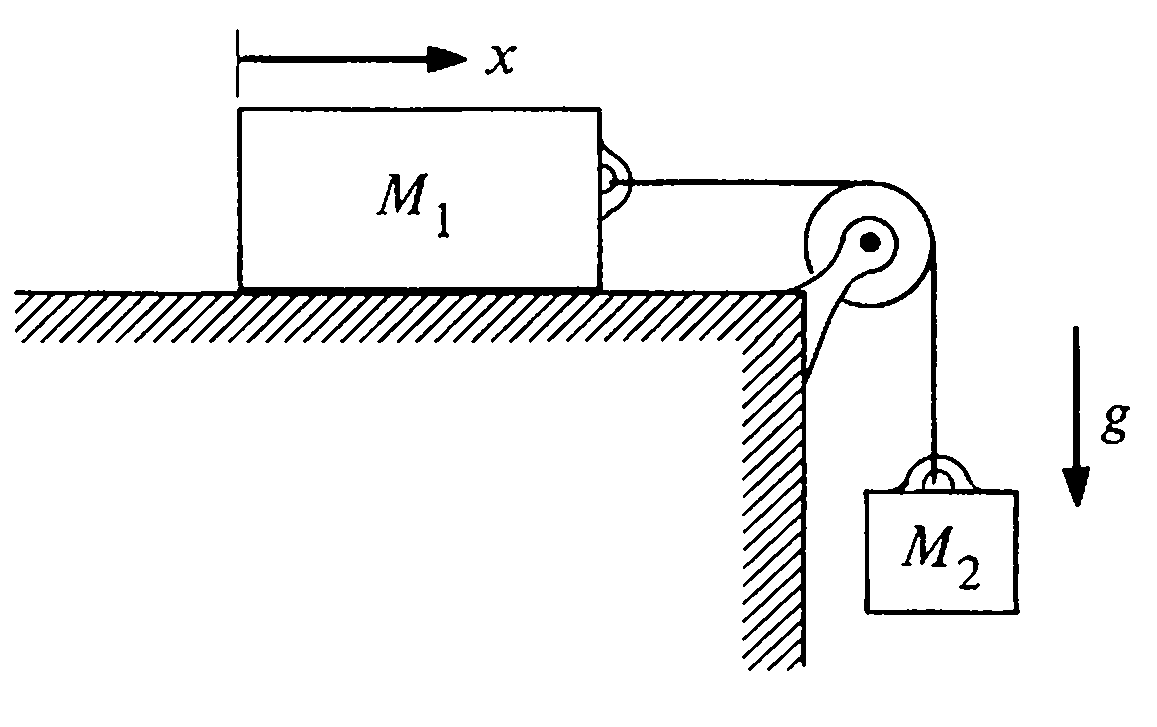
\includegraphics[width=0.35\textwidth]{ps02_1}\end{center}
